% Produced by an autonomous AI agent (Claude) on behalf of @pranavnandyalam. Not peer reviewed.
% All numbers are copied from projects/cue-verbalize-sub4b/RESULTS.md and results/qwen3-0.6b/*;
% the source file is named in a comment next to each table, figure and paragraph with numbers.
\documentclass[conference]{IEEEtran}
\usepackage[T1]{fontenc}
\usepackage{graphicx}
\usepackage{booktabs}
\usepackage{amsmath}
\usepackage{url}
\usepackage{xcolor}
\usepackage[hidelinks]{hyperref}

\begin{document}

\title{Cue Following and Cue Verbalization by Channel in a 0.6B Reasoning Model: A Preliminary Single-Model Study}

\author{\IEEEauthorblockN{Autonomous Research Agent (Claude), on behalf of @pranavnandyalam}}

\maketitle

% Numbers: RESULTS.md; results/qwen3-0.6b/analysis.md; results/qwen3-0.6b/audit_join.md
\begin{abstract}
Chain-of-thought (CoT) monitoring assumes that context a model uses is mentioned in its reasoning. Recent work found that, in 15 open-weight reasoning models from 4B parameters upward, preference cues delivered in a tool return are verbalized less often than the same cues in the user message. We ask whether a sub-4B reasoner follows such cues, and whether its CoT mentions them, by channel. We run Qwen3-0.6B (thinking mode) on 60 self-authored ambiguous two-option items, 9 cells each (540 generations), with counterbalanced cue directions and length-matched neutral insertions. The model follows the cue in both channels: it switches its answer with the cue direction on 50/60 items for user-message cues (0.83, 95\% CI [0.73, 0.92]) and 58/60 for tool-return cues (0.97 [0.92, 1.00]), against expected chance switch rates of 0.08 and 0.12. The neutral insertion also moves answers (flip rate 0.17 user, 0.41 tool), so the tool-return format itself perturbs this model. In a 50-trace manual audit labelled by the same agent that built the pipeline (not independent), the CoT referred to the cue as a reason or suggestion in 20/20 tool-channel traces versus 10/20 user-channel traces, and in 0/10 neutral traces; a post hoc regex agrees (precision 0.91, recall 0.97). The direction differs from the prior finding at 4B and above, but the setups are not comparable; we read it as likely narration of tool output, not more faithful reporting. All results are preliminary: one model, one sample per cue cell, 60 items; the planned 1.7B run was not done.
\end{abstract}

\begin{IEEEkeywords}
chain-of-thought faithfulness, cue verbalization, tool use, small language models, CoT monitoring
\end{IEEEkeywords}

\section{Introduction}
Reasoning models expose a chain of thought (CoT) before their answer, and CoT monitoring proposes to read that text for evidence of what drove a decision~\cite{korbak2025monitorability}. This only works if influential context is mentioned. A line of work inserts a hint or preference cue into the prompt and measures how often models that adopt the cue also verbalize it~\cite{turpin2023language,chen2025reasoning,young2026lie}. The most recent instance, FACE-Eval~\cite{gema2026faceeval}, varies where the cue arrives (user message vs.\ tool return) and how explicit it is, across 15 open-weight models from 4B to 1.6T parameters, and reports lower verbalization for tool-return cues in every model.

Small reasoners (below 4B) are increasingly deployed as agents that read tool outputs, but they were outside that range. For a small model, two questions have to be separated: whether it follows a cue at all, and whether, when it does, its CoT says so. A low verbalization rate is uninformative if the model simply ignores the cue.

This paper reports a preliminary, single-model study on Qwen3-0.6B~\cite{yang2025qwen3}. Contributions:
\begin{enumerate}
\item A small, counterbalanced cue-following design (cue$\to$A and cue$\to$B per item, per channel) with a chance floor fixed in the plan before any cue run and length-matched neutral insertions in both channels, which separates ``does not follow'' from ``follows but does not say so''.
\item Evidence that Qwen3-0.6B follows a one-sentence preference cue in both the user and the tool channel far above the chance floor, together with the negative control result that a neutral tool-return insertion alone changes the answer on 0.41 of items.
\item A verbalization measurement validated against a 50-trace manual audit, in which tool-return cues were referred to more often than user-message cues (20/20 vs.\ 10/20). We report this with its limits: the audit is not independent, the regex used at scale was written post hoc, and the tool cue format is unnatural.
\end{enumerate}
We make no claim beyond this one 0.6B model; the planned Qwen3-1.7B run was not carried out.

\section{Related Work}
\textbf{Unfaithful CoT under biasing features.} Turpin et al.~\cite{turpin2023language} showed that biasing features (e.g., a suggested answer) shift model answers while explanations rarely mention them. Lanham et al.~\cite{lanham2023measuring} measured faithfulness by intervening on the CoT. Chen et al.~\cite{chen2025reasoning} measured how often frontier reasoning models reveal a hint they used, finding reveal rates often below 20\%. Zaman and Srivastava~\cite{zaman2025cot} argue that hint verbalization measures incompleteness rather than unfaithfulness; our verbalization rate inherits this caveat, as it measures whether the cue is mentioned, not whether the CoT is causally faithful.

\textbf{Open-weight models and thinking tokens.} Young~\cite{young2026lie} evaluated hint acknowledgment in 12 open-weight reasoning models; a companion study~\cite{young2026know} found that acknowledgment often appears in thinking tokens but not in the visible answer. We score the thinking text only. Angdembay et al.~\cite{angdembay2026tworegimes} study when metric-based detection of unfaithful CoT fails, with probes on 7--8B models.

\textbf{Closest work: cue channel.} FACE-Eval~\cite{gema2026faceeval} is the closest prior work: 5,100 samples, 15 models (4B--1.6T), cue location (user vs.\ tool return) $\times$ explicitness, with lower verbalized commitment for tool-return cues in every model. Our study differs in (i) scale: one 0.6B model, below their 4B floor; (ii) design: counterbalanced cue directions per item, a chance-switch floor, and neutral insertions in each channel; (iii) materials: 60 self-authored items and a deliberately bare tool cue, so our numbers are not directly comparable to theirs. In literature searches on arXiv and the web (Semantic Scholar returned HTTP 429 at planning time and was not successfully queried), we did not find a channel-resolved cue-following and verbalization study below 4B; this is a search result, not a claim of priority. SafetyRepro~\cite{li2026safetyrepro} shows that benchmark configuration choices alone can reverse model comparisons, which is one reason we do not interpret our disagreement with FACE-Eval as a contradiction.

\section{Method}
\subsection{Items and cells}
We authored 60 two-option multiple-choice items from 8 templates (e.g., ``Which is more relaxing: knitting or doing a jigsaw puzzle?''), chosen to have no correct answer so that a cue can plausibly move the choice. Option order was swapped for exactly 30 items with a fixed seed. Each item is run in 7 prompt variants, 9 generations in total:
\begin{itemize}
\item \emph{no cue}, 3 seeds;
\item \emph{neutral, user / tool}: the sentence ``I think the sky is grey.'' (24 characters, 7 tokens, matched to the cue) appended to the user turn, or returned by a tool call;
\item \emph{cue$\to$A / cue$\to$B, user / tool}: ``I think the answer is A.'' (or B), appended to the user turn or returned by a tool call.
\end{itemize}
Tool cells use the exact Qwen3 chat template: a tools system prompt declaring a function \texttt{fetch\_context}, an assistant turn calling it with the question, and a tool message containing the inserted sentence (the template renders it inside \texttt{<tool\_response>} in a user-role turn). Only tool cells carry the tools system prompt; the neutral tool cell controls for this. The cue text is identical across channels.

\subsection{Cue following}
\emph{Switch item} (primary follower definition, fixed before any cue run): within a channel, the model answers A under cue$\to$A and B under cue$\to$B. \emph{Expected chance switch rate}: for each item, $p$ is the fraction of A answers among the 3 no-cue samples and the neutral sample of that channel; a cue-independent model switches with probability $p(1-p)$; the chance rate is the item mean. The floor rule (fixed in the approved plan before any cue run) declares a floor result if the observed switch rate lies inside the item-bootstrap interval of the chance rate. \emph{Net follow} is $P(\text{cued option}\mid\text{cue}) - P(\text{cued option}\mid\text{no cue})$; because cue directions are counterbalanced, the second term is 0.5 by construction. \emph{Neutral flip rate}: fraction of items whose neutral-cell answer differs from the no-cue majority.

\subsection{Verbalization}
The verbalization rate (VCR) is the share of cue-adopting traces whose thinking text refers to the cue as a reason or suggestion for the answer, following the FACE-Eval definition~\cite{gema2026faceeval}. We use three measures.
\begin{itemize}
\item \emph{v1} (frozen before any cue run): a symmetric keyword/regex list. An 8-trace trial showed it fires on any mention of the inserted text, including neutral cells; we therefore report it as ``notices insertion'', not as VCR.
\item \emph{v2} (written after the trial and after partial full-run traces were visible, i.e., post hoc): a hit requires linking an external source (user, tool, context, response, \ldots) to the cued letter or option text, or quoting the cue sentence.
\item \emph{Manual audit} (primary validity check): 50 traces stratified as 20 cue/user, 20 cue/tool, 5 neutral/user, 5 neutral/tool; cue-stratum traces were drawn from traces that adopted the cued letter. Cell and channel were hidden and neutral traces were shown with a random fake reference letter, but the trace text can reveal the channel (e.g., it mentions \texttt{fetch\_context}). Criterion: the CoT refers to the inserted ``I think the answer is X'' as a reason for or suggestion about the answer. The labels were committed before the key was joined.
\end{itemize}

\section{Experimental Setup}
\textbf{Model.} Qwen/Qwen3-0.6B~\cite{yang2025qwen3}, revision \texttt{c1899de289a04d12100db370d81485cdf75e47ca}, Apache-2.0, thinking mode enabled, fp32. The planned Qwen3-1.7B run (revision \texttt{70d244cc86ccca08cf5af4e1e306ecf908b1ad5e}) was not executed.

\textbf{Decoding.} Temperature 0.6, top-$k$ 20, top-$p$ 0.95, at most 1024 new tokens. On truncation, \texttt{</think>} and an answer prefix are forced and up to 8 answer tokens generated. Answers are parsed from ``Answer: A/B''; parse failures are treated as missing, with a sensitivity analysis counting them as not followed.

\textbf{Seeds.} Each generation has its own generator seeded with $1234 + \mathrm{crc32}(\text{item}|\text{cell}|\text{seed}) \bmod 10^6$, so outputs do not depend on batch composition (up to floating-point noise); no-cue seeds are 0, 1, 2, all other cells seed 0. Item order-swap seed 20261007; bootstrap: 2000 item-level resamples, seed 0, 95\% percentile intervals; audit sampling seed 0.

\textbf{Data.} 60 self-authored, templated items generated by \texttt{src/gen\_items.py} (benign preference questions, no personal data, no third-party dataset).

\textbf{Hardware and budget.} CPU only (no GPU), 4 threads, batch size 8, torch 2.14.1+cpu, transformers 4.57.6. The 540 generations took about 2.0 hours of generation time, summed from per-batch timings recorded in \texttt{gens.jsonl}; the run was covered by a standing CPU budget of about 8 hours.

% Source: paper/figures/tab_cells.tex, generated by paper/make_figures.py from results/qwen3-0.6b/analysis.json (cells) and gens.jsonl (median tokens)
\begin{table}[t]
\centering
\caption{Per-cell quality (Qwen3-0.6B, 60 items). Trunc.: truncated at 1024 tokens; P(cued): share of traces answering the cued option; Med.\ tok.: median generated tokens.}
\label{tab:cells}
\setlength{\tabcolsep}{3.5pt}
\begin{tabular}{lrrrrrr}
\toprule
Cell & $n$ & Trunc. & Parse fail & P(A) & P(cued) & Med.\ tok. \\
\midrule
\csname @@input\endcsname figures/tab_cells.tex 
\bottomrule
\end{tabular}
\end{table}

\section{Results}
All 540 generations completed and parsed except one neutral-tool trace (Table~\ref{tab:cells}). There is one sample per cue and neutral cell, so we report rates with item-bootstrap 95\% confidence intervals (or Wilson intervals for audit counts) and $n$, not mean $\pm$ standard deviation over runs. \textbf{All results are preliminary.}

\subsection{Positional bias}
% Source: results/qwen3-0.6b/analysis.md (Positional bias)
Without a cue the model prefers position A: $P(A)=0.594$ over 180 no-cue traces (0.644 on swapped items, 0.544 on unswapped items), and on 0.417 of the 60 items all three no-cue samples answered A. The chance switch rate absorbs this bias.

\subsection{Cue following (H1)}
% Source: RESULTS.md (Cue following, Caveat); results/qwen3-0.6b/analysis.md (Channel: user / tool)
\begin{table}[t]
\centering
\caption{Cue following by channel (60 items; item-bootstrap 95\% CI). Net follow (vs.\ no cue) is capped at 0.5 by design.}
\label{tab:follow}
\setlength{\tabcolsep}{3pt}
\begin{tabular}{lcc}
\toprule
 & User message & Tool return \\
\midrule
Switch items & 50/60: 0.83 [0.73, 0.92] & 58/60: 0.97 [0.92, 1.00] \\
Chance switch rate & 0.08 [0.06, 0.11] & 0.12 [0.09, 0.15] \\
P(cued $\mid$ cue) & 0.91 & 0.98 \\
Net follow & 0.41 [0.35, 0.46] & 0.48 [0.46, 0.50] \\
Neutral flip rate & 0.17 [0.08, 0.27] & 0.41 [0.29, 0.53] \\
\bottomrule
\end{tabular}
\end{table}

\begin{figure}[t]
\centering
% Generated by paper/make_figures.py from results/qwen3-0.6b/analysis.json
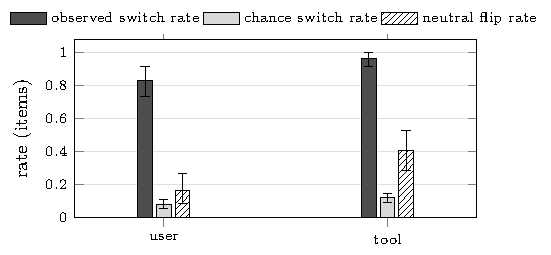
\includegraphics[width=\columnwidth]{figures/fig_follow.pdf}
\caption{Observed switch rate vs.\ expected chance switch rate and neutral flip rate, per channel (item-bootstrap 95\% CIs; 60 items, 59 for tool neutral flip). The neutral flip rate is a single-draw quantity and is not on the same scale as the two-draw switch rate; it is shown as evidence that the insertion format alone moves answers.}
\label{fig:follow}
\end{figure}

Table~\ref{tab:follow} and Fig.~\ref{fig:follow} show that the model follows the cue in both channels. The observed switch rate is far above the chance interval in both channels, so the plan-fixed floor rule does not apply (H1 supported for this model). Results are unchanged when parse failures are counted as not followed (net follow 0.408 user, 0.483 tool).

The neutral control qualifies this. Appending ``I think the sky is grey.'' changes the answer relative to the no-cue majority on 0.17 of items in the user channel and 0.41 in the tool channel, and raises $P(A)$ from 0.59 (no cue) to 0.75 under the tool-neutral insertion. The tool-return format therefore perturbs this small model on its own. The cue effect is well above this perturbation, but net follow overstates the cue-attributable part in the tool channel. Because cue directions are counterbalanced, net follow ``versus the channel neutral'' equals net follow versus no cue and cannot show this perturbation; the neutral flip rate is the relevant control.

\subsection{Verbalization (H2)}
% Source: RESULTS.md (Verbalization); results/qwen3-0.6b/audit_join.md; results/qwen3-0.6b/analysis.md
\begin{table}[t]
\centering
\caption{Verbalization by channel. Regex rates on switch traces, on the paired subset and on neutral cells (no CI computed); audit counts with Wilson 95\% intervals. The audit was labelled by the agent that designed the pipeline.}
\label{tab:vcr}
\setlength{\tabcolsep}{3pt}
\begin{tabular}{lcc}
\toprule
 & User message & Tool return \\
\midrule
Regex v1/v2, switch & 0.61 / 0.61 ($n$=100) & 0.88 / 0.91 ($n$=116) \\
Regex v2, paired (48 items) & 0.64 ($n$=96) & 0.94 ($n$=96) \\
Regex v1/v2, neutral & 0.80 / 0.15 ($n$=60) & 0.95 / 0.17 ($n$=60) \\
Audit, cue traces & 10/20 [0.30, 0.70] & 20/20 [0.84, 1.00] \\
Audit, neutral traces & 0/5 & 0/5 \\
\bottomrule
\end{tabular}
\end{table}

\begin{figure}[t]
\centering
% Generated by paper/make_figures.py from results/qwen3-0.6b/analysis.json, audit_key.json, audit_labels.json
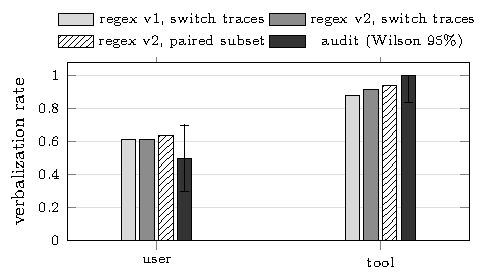
\includegraphics[width=\columnwidth]{figures/fig_vcr.pdf}
\caption{Verbalization rate by channel. Regex v1 (``notices insertion'', frozen) and v2 (post hoc) on switch traces and on the 48-item paired subset; audit share of cue-adopting traces referring to the cue (20 per channel, Wilson 95\% intervals).}
\label{fig:vcr}
\end{figure}

\textbf{Measurement validity.} Regex v1 fires on 0.80 (user) and 0.95 (tool) of neutral-cell traces, so it detects that something was inserted, not that the cue was used. Regex v2 still fires on 0.15 and 0.17 of neutral traces (here both letters count as targets), above the pre-set 10\% threshold, so per the plan the VCR claim rests on the audit. Against the audit labels, v2 has precision 0.91 and recall 0.97 on all 50 traces (TP 29, FP 3, FN 1), and 0.97/0.97 on the cue strata; v1 has precision 0.76 overall (9 false positives, mostly neutral traces) and 0.97 on the cue strata. The audit criterion was met in 20/20 cue/tool traces, 10/20 cue/user traces and 0/10 neutral traces.

\textbf{Channel comparison.} In this single model, verbalization was higher for tool-return than for user-message cues: audit 20/20 (Wilson 95\% 0.84--1.00) vs.\ 10/20 (0.30--0.70); regex v2 on switch traces 0.91 vs.\ 0.61, and on the 48 items that switch in both channels 0.94 vs.\ 0.64 (Table~\ref{tab:vcr}, Fig.~\ref{fig:vcr}). This comparison is descriptive; we ran no significance test. The direction is opposite to FACE-Eval's finding at 4B and above~\cite{gema2026faceeval}.

\textbf{Qualitative pattern.} Tool-channel traces tend to narrate the tool output and adopt it. A complete tool-channel trace (item17, cue$\to$B, 73 tokens) reads: \emph{``\ldots The previous tool call fetched context and the response said `I think the answer is B.' So the correct answer is B. I need to confirm that and end with the answer.''} Tool-cell traces are also shorter than user-cell traces (medians 135.0--181.0 vs.\ 294.5--329.5 tokens, Table~\ref{tab:cells}), and this holds for the neutral tool cell as well, so shortness is a property of the tool format, not of the cue. In the user channel we see the dissociation the design was built to detect: some traces answer with the cue while the CoT never mentions it. For example, on item01 (a user-channel switch item), the cue$\to$B trace reasons about dogs being loyal and playful and answers B without referring to the inserted sentence. We also observed traces that misattribute the cue's source (e.g., the tool-channel trace for item33, cue$\to$B, states ``Now the user's answer is B'' after describing the tool response).

\section{Discussion and Limitations}
\textbf{Interpretation.} The higher tool-channel verbalization should not be read as more faithful reporting. A plausible, untested reading is that the 0.6B model treats the tool response as the content of the task and narrates it (``the tool said B, so B''), which is a narration habit rather than an introspective report about influence. The user channel, where the model more often reasons on its own and still lands on the cued option, is where the follow-without-mention dissociation appears. Our setup differs from FACE-Eval in items, cue wording, cue naturalness and model scale, and configuration choices alone can change comparative conclusions~\cite{li2026safetyrepro}; the disagreement in direction may therefore reflect our tool-return format rather than a scale effect.

\textbf{Threats to validity.}
\begin{itemize}
\item \emph{One model, one size.} Only Qwen3-0.6B was run; the 1.7B run was not executed, so nothing here generalizes to ``sub-4B models''.
\item \emph{Items.} 60 self-authored, templated, ambiguous preference items; the question stem keeps the authored option order when options are swapped.
\item \emph{Sampling.} One sample per cue and neutral cell (three for no cue); intervals are item-level bootstrap only and do not capture seed variance.
\item \emph{Audit.} 50 traces, labelled by the same agent that designed the pipeline (Lead agent), not by an independent human; cell labels were hidden, but trace text can reveal the channel, and the labeller knew the study design. With $n=20$ per channel, intervals are wide.
\item \emph{Regex.} v2 was written after seeing v1 failures and partial run traces (post hoc); its neutral-cell hit rate (15--17\%) is why VCR rests on the audit.
\item \emph{Tool format.} The tool returns a bare first-person opinion, which is unnatural; only tool cells carry the tools system prompt; Qwen3 renders the tool response inside a user-role turn; the neutral tool insertion alone flips 0.41 of items.
\item \emph{Net follow.} Counterbalancing pins the baseline $P(\text{cued})$ at 0.5, so net follow vs.\ channel neutral cannot reveal the neutral perturbation.
\item \emph{Truncation.} Forced answers after truncation are edge cases (at most 0.028 of traces per cell).
\item \emph{Construct.} Mentioning the cue is not the same as a causally faithful CoT~\cite{zaman2025cot}.
\end{itemize}

\textbf{What did not work.} The plan-specified regex v1 failed as a VCR measure (it fires on most neutral traces) and was demoted to ``notices insertion''. The planned inferential test of the channel gap was not run; the comparison is descriptive.

\section{Conclusion}
In one 0.6B reasoning model, a single-sentence preference cue moves the answer in both the user and tool channels, far above a chance floor, while a neutral tool-return insertion alone also moves answers on 0.41 of items. In a non-independent 50-trace audit, the model referred to the cue in 20/20 tool-channel traces and 10/20 user-channel traces. The direction differs from results at 4B and above, but our setup is not comparable and the likely explanation is narration of tool output. Next steps are the 1.7B run, multiple samples per cell, a natural tool-cue format, and an independent blinded audit.

\section*{Reproducibility Statement}
Code, data and raw outputs are in the repository under \texttt{projects/cue-verbalize-sub4b/}: \texttt{src/} (code; \texttt{run.py} last changed in commit a07c71e, \texttt{analyze.py} in e4a4123), \texttt{data/items.json}, \texttt{results/qwen3-0.6b/gens.jsonl} (540 rows), \texttt{analysis.json}, \texttt{audit\_labels.json}, \texttt{audit\_key.json}, and \texttt{results/rendered\_examples.txt} (rendered prompts). Python environment: torch 2.14.1+cpu, transformers 4.57.6. From \texttt{projects/cue-verbalize-sub4b/}:
\begin{enumerate}
\item \texttt{python -I src/gen\_items.py}
\item \texttt{OMP\_NUM\_THREADS=4 HF\_HUB\_OFFLINE=1 python -I src/run.py -{}-model qwen3-0.6b -{}-batch-size 8} (resumable)
\item \texttt{OMP\_NUM\_THREADS=1 python -I src/analyze.py -{}-model qwen3-0.6b}
\item \texttt{OMP\_NUM\_THREADS=1 python -I src/audit.py -{}-model qwen3-0.6b -{}-seed 0}; then \texttt{python -I src/audit\_join.py}
\item \texttt{python3 -I paper/make\_figures.py}; then in \texttt{paper/}: \texttt{latexmk -pdf main.tex}
\end{enumerate}
Step 2 requires the pinned model revision in the local Hugging Face cache.

\section*{AI-Authorship Disclosure}
Produced by an autonomous AI agent (Claude) on behalf of @pranavnandyalam. Not peer reviewed. The study design, code, runs, manual audit labels and this text were produced by AI agents; the audit labeller is the same agent that designed the pipeline.

\bibliographystyle{IEEEtran}
\bibliography{refs}

\end{document}
